\chapter{Raspberry Pi Setting}
\label{chp:rpi}

\section{About Raspberry Pi}
\par The \gls{rpi} is a credit-card-sized single-board computer developed in the UK by the Raspberry Pi Foundation with the intention of promoting the teaching of basic computer science in the schools. \cite{rpi} The \gls{rpi} has a Broadcom BCM2835 system on a chip, which includes an ARM1176JZF-S 700 MHz processor (The firmware includes a number of "Turbo" modes so that the user can attempt overclocking, up to 1 GHz, without affecting the warranty), VideoCore IV GPU, and was originally shipped with 256 megabytes of RAM, later upgrade to 512 MB. It does not include a built-in hard disk or solid-state drive, but uses an \gls{sd} card for booting and long-term storage.

\subsection{\gls{rpi} Hardware for Project}
\par In this project, one Kingston 8 \gls{gb} \gls{sd} card is used instead of Samsung 16 \gls{gb} \gls{sd} card in previous master project\cite{TorgeirMR} because the Samsung 16 \gls{gb} \gls{sd} card used in the previous project is quite unstable since its root file system has been broken by the voltage changes of the \gls{usb} hub on the \gls{rpi} during the development of this report project. 
\par In this project, it will use model B as the residential access point because the model B is more powerful on the hardware than the model A, and it has two built in integrated \gls{usb} ports. Since the residential access point need provide the Wifi hot-spot function for other client user to connect to, and the normal \gls{rpi} is not equited with on-board Wifi block component, a compatible D-link DWL-G122 would be used with \gls{rpi} by the \gls{usb} connecting.
\begin{figure}
	\centering
    	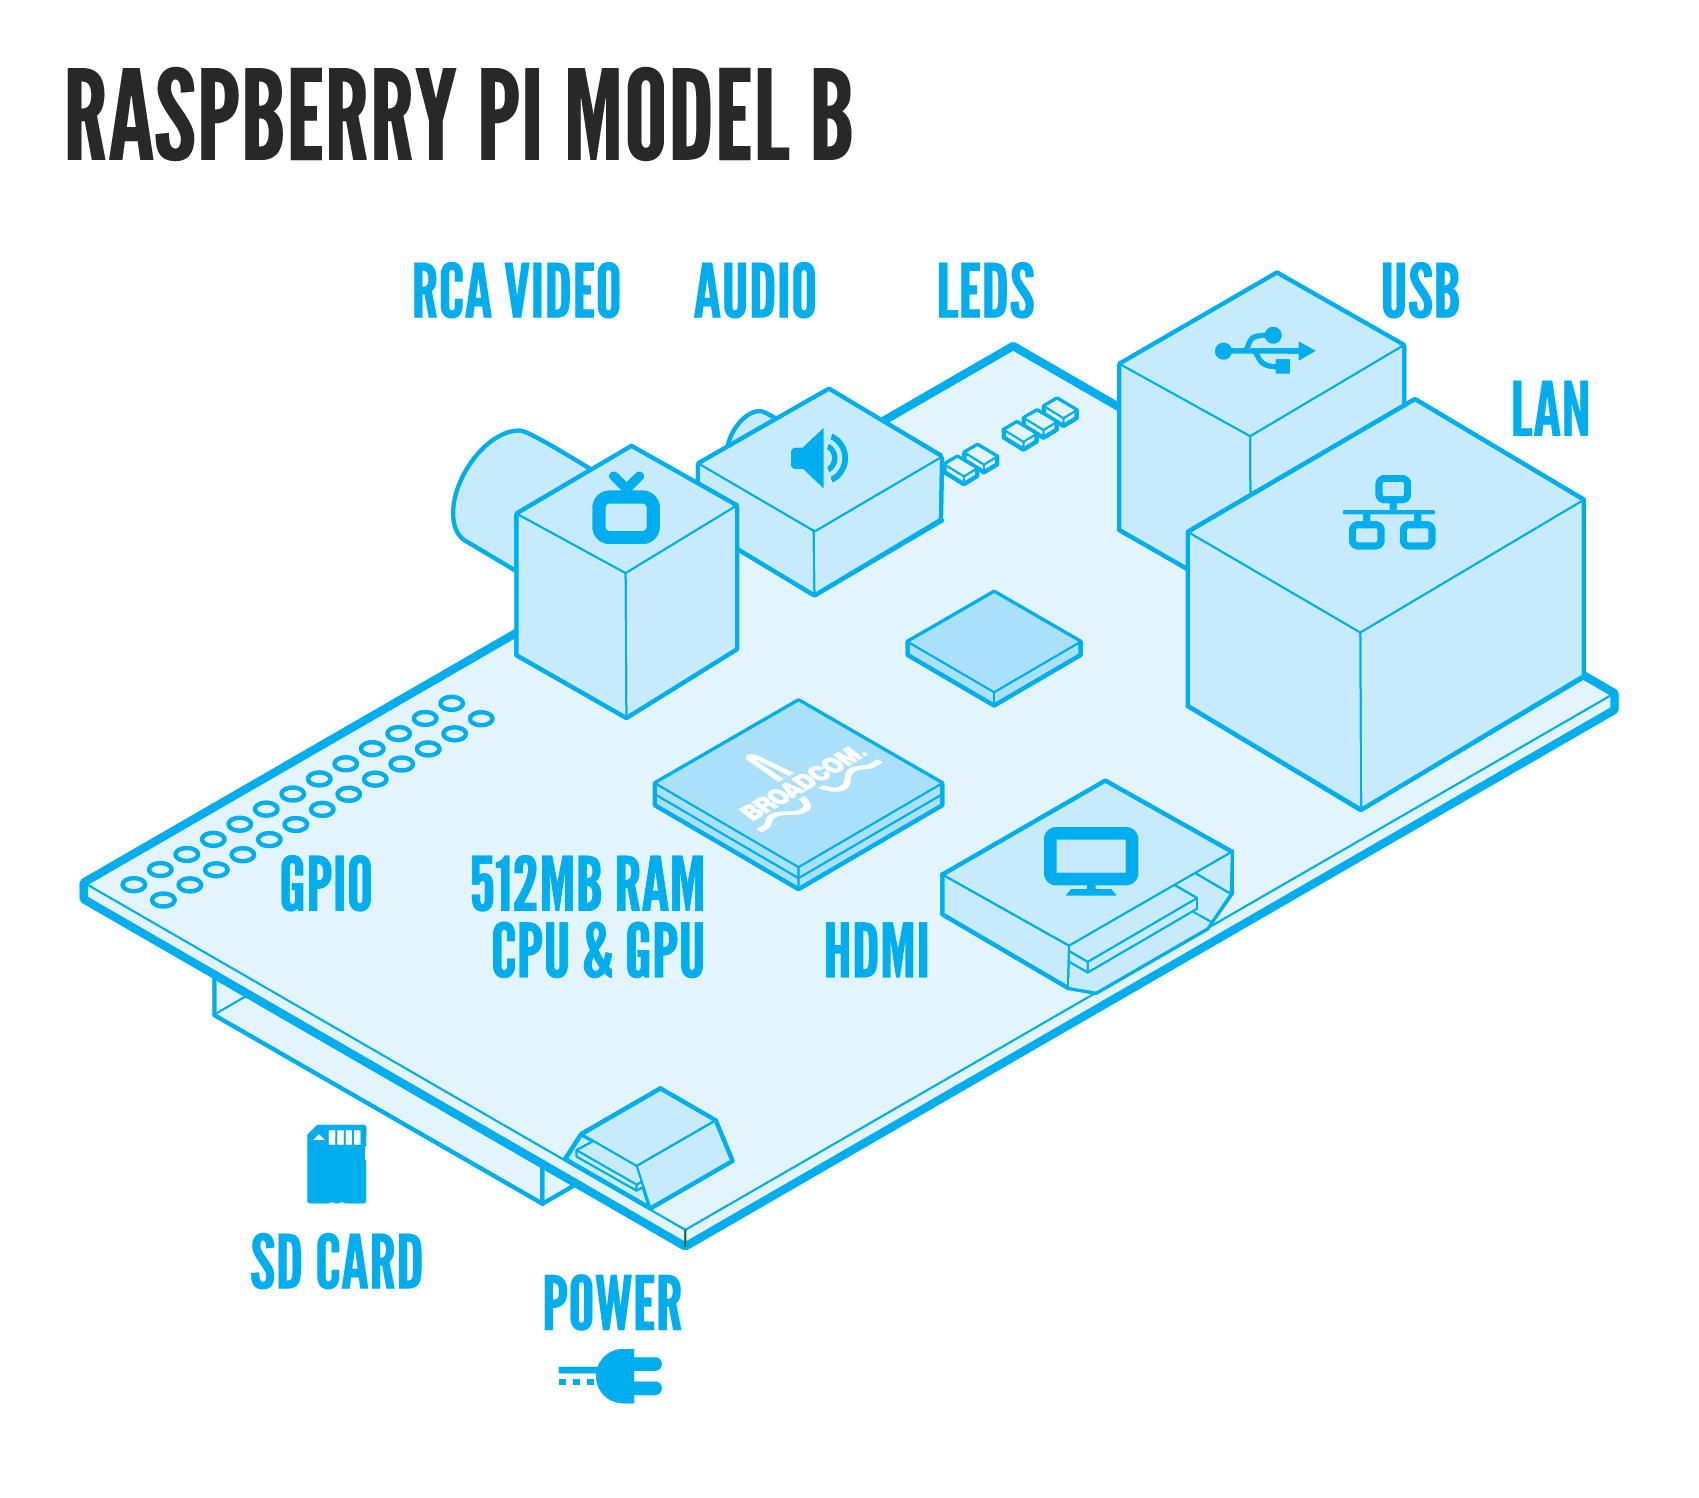
\includegraphics[width=0.80\textwidth,natwidth=610,natheight=642]{figs/RaspiModelB.png}
  	\caption{Raspberry Pi used as Residential access point}
  	\label{fig:rpi}
\end{figure}

\subsection{\gls{rpi} Operation System}
\par The Raspberry Pi Foundation provides Debian and Arch Linux ARM distributions as \gls{rpi} operating system.Tools are available for Python as the main programming language on the \gls{rpi}, with support for BBC BASIC (via the RISC OS image or the "Brandy Basic" clone for Linux),C and Perl. In this project the recommended operating system, Raspbian wheezy\cite{raspbian} will be used as \gls{rpi} operating system. Raspbian is a free operating system based on Debian optimized for the Raspberry Pi hardware. An operating system is the set of basic programs and utilities that make Raspberry Pi run. However, Raspbian provides more than a pure OS: it comes with over 35,000 packages, pre-compiled software bundled in a nice format for easy installation on Raspberry Pi. For this prototype project, this kind of beginner operating system is the best choice.

\section{Applications Using on Raspberry Pi}

\subsection{hostapd}
\par Most using package to provide Wifi hot-spot function on \gls{rpi} is hostapd\cite{hostapd} package. hostapd is an \gls{ieee} 802.11 \gls{ap} and \gls{ieee} 802.1X/\gls{wpa}/\gls{wpa2}/\gls{eap}/\gls{radius} Authenticator. The  advantages of using hostapd are that it is compatible well with the \gls{rpi} and it is easy to manually modified by script configuration file. The setting up configuration file is shown in Code Snippet\ref{code:hostapd_config}.

\begin{algorithm}[h]
\floatname{algorithm}{Code Snippet}
  \caption{hostapd configuration file}
  \label{code:hostapd_config}
  \begin{verbatim}
  
interface=wlan0
driver=nl80211
ctrl_interface=/var/run/hostapd
ctrl_interface_group=0
ssid=raspberry
hw_mode=g
channel=8
wpa=0
beacon_int=100
auth_algs=1
wmm_enabled=1
 \end{verbatim}
\end{algorithm}

\subsection{\gls{dhcp}}
\par For dynamically allocating \gls{ip} address for connected clients with \gls{rpi}, the protocol, \gls{dhcp} \cite{dhcp} is using in this project. \gls{dhcp} is a standardized networking protocol used on \gls{ip} addresses and other information that is needed for internet communication.\gls{dhcp} allows computers and other devices to receive an \gls{ip} address automatically from a central \gls{dhcp} server(\gls{rpi} in this project), reducing the need for a network administrator or a user from having to configure these settings manually. This working process is fit the requirement of prototype project because client users need have a \gls{ip} address to have the access to post internet access request to the central server and wait for the response. And the recommended networking protocol using in this case from the \gls{rpi} community is \gls{dhcp}.
\subsection{Dnsmasq}
\par In this project, on \gls{rpi} device, an application named dnsmasq \cite{dnsmasq} will be used to provide \gls{dns} forwarder and \gls{dhcp} server. For this prototype project, dnsmasq is a lightweight, easy to configure \gls{dns} forwarder and \gls{dhcp} server. It is designed to provide \gls{dns} and, optionally, \gls{dhcp}, to a small network, like the residential area wireless network in this project case.

\begin{algorithm}[h]
\floatname{algorithm}{Code Snippet}
  \caption{dnsmasq configuration}
  \label{code:dnsmasq_config}
  \begin{verbatim}
  
interface=wlan0

dhcp-range=unauth,10.0.0.65,10.0.0.94,2m
dhcp-option-force=unauth,1,255.255.255.224
dhcp-option-force=unauth,6,129.241.200.170,129.241.200.170

dhcp-range=auth,10.0.0.1,static,2m
dhcp-range=auth,10.0.0.2,10.0.0.63,2h
dhcp-option-force=auth,1,255.255.255.192
dhcp-option-force=auth,6,8.8.8.8,8.8.4.4

dhcp-hostsfile=/etc/dnsmasq.hosts
 \end{verbatim}
\end{algorithm}

\par The configuration file for dnsmasq is shown in Code Snippet \ref{code:dnsmasq_config}. For this project, we set unauthenticated \gls{ip} addresses in the range from 10.0.0.65 to 10.0.0.94, the the lease available time is two minutes. On the other hand, the authenticated \gls{ip} addresses are in the range from 10.0.0.2 to 10.0.0.62. And for unauthenticated clients, the \gls{dns} server would be 129.241.200.170 which is central management server to redirect network traffic for each unauthenticated \gls{ip} address. For authenticated clients, the \gls{dns} server would be the Google Open \gls{dns} server(8.8.8.8,8.8.4.4) to reduce the complexity of the \gls{rpi} residential access point. Moreover, we set the hosts file to '/etc/dnsmasq.hosts'. this file will store the static lease script. The example script in dnsmasq.hosts would be like Code Snippet \ref{code:dnsmasq_hosts}, it includes \gls{ip} address leased by the client user , \gls{macaddress} address from the client user device and the \gls{ip} lease available time. The dnsmasq hosts file would be modified when there is any changes from the central management server updating the client user authorization. 
\begin{algorithm}[h]
\floatname{algorithm}{Code Snippet}
  \caption{dnsmasq dhcp host format}
  \label{code:dnsmasq_host_format}
  \begin{verbatim}
--dhcp-host=[<hwaddr>][,<ipaddr>][,<lease_time>][,ignore]
 \end{verbatim}
\end{algorithm}
\par There is a bug in the previous master project report \cite{TorgeirMR}, which is the format of the \gls{ip} address lease is not correct when there is an authenticated client which needs to be added to as static lease in dnsmasq hosts file. The format of the dhcp host should be the format as Dnsmasq dhcp host format shown in Code Snippet \ref{code:dnsmasq_host_format} according to dnsmasq document\cite{dnsmasq_doc}. Then the bash script for adding static lease in the dnsmasq host file need to be fixed because of this bug. There are two files to place the leases for connecting devicees managed by dnsmasq. One is to store the static lease information, dnsmasq.hosts (/etc/dnsmasq.hosts), the other is to store the temporary lease information, dnsmasq.leases (/var/lib/misc/dnsmasq.leases). This project is using both files to change the \gls{ip} address for request clients. This will be discuss more detail in the bash shell scripts in the section\ref{sec:scripts_rpi}.

\begin{algorithm}[h]
\floatname{algorithm}{Code Snippet}
  \caption{dnsmasq hosts file}
  \label{code:dnsmasq_hosts}
  \begin{verbatim}
  
e4:ce:8f:03:7f:e0,10.0.0.6,2h
 \end{verbatim}
\end{algorithm}

\subsection{Iptables}
\par After user client gets the \gls{ip} address from the residential access point, the residential access point need provide a way for user client to get the authenticated \gls{ip} and set the authenticated \gls{ip} with the new routing policy. In this project, iptables\cite{iptables} is used to set new routing policy. Iptables is a user space application program that allows a system administrator to configure the tables provided by the Linux kernel firewall and the chains and rules it stores. Different kernel modules and programs are currently used for different protocols; iptables applies to IPv4, ip6tables to IPv6, arptables to \gls{arp}, and ebtables to Ethernet frames.
\par When a \gls{ip} packet arives at the residential access point (\gls{rpi}), it is sequentially checked against the rules in the iptables. The main tables in iptables are filter, nat and mangle. Each table contains a number of chains and each chain has a set of rules. The working process of manipulating iptables will not be covered in this report since it is fully described in previous master project report \cite{TorgeirMR}.

\section{Scripts on Raspberry Pi}
\label{sec:scripts_rpi}
\par On \gls{rpi} residential access point, the main function to manipulate Iptables and configure dnsmasq is based on the shell scripts on the \gls{rpi}. And the commands are got from the central management server by the python scripts \gls{http} post request which running repeatedly in 60 milliseconds interval.Also the proxy server hosting is based on python scripts hosting on the port 8089, the iptables rules to force unauthenticated devices redirect to this hosting port is shown in Code Snippet \ref{code:iptables_setup} of Appendix \ref{chp:appendix}. Because of the time limit, in this project, it will use the same mechanism on \gls{rpi} as previous master project \cite{TorgeirMR}, other possible solution will be discussed in Chapter \ref{chp:future_work}. However, there are several bugs in the master project report provided, which is fixed in this project to make \gls{rpi} residential access point working. In this section,we will discuss these fix changes, the original and correct part from previous master project is not included.
\subsection{RPI Configuration Python Script}
\par On the \gls{rpi} residential access point, \gls{rpi} need to run two important python scripts to make the residential access point work in the whole internet access control system. One is transproxy.py script which is the same transproxy.py python script on the Github repository (\url{https://github.com/TorgeirCook/RPIConfigurationServer/blob/master/transproxy.py}), it is developed by Torgeir Pedersen Cook in his master project. This python script is to host the proxy server on port 8089 of \gls{rpi} to make sure all the redirected network traffic will reach the remote central management server for unauthenticated \gls{ip} address client user to request internet access and also to get the current connected device \gls{macaddress} address.The proxy server hosting python script is on the Github repository (\url{https://github.com/br1anchen/WifiAccess_RPIConfigurationServer/blob/master/transproxy.py}) since it has not been any changes from previous master project then it will not be further discussed in this report.
\par Another script running on \gls{rpi} is configserver.py script, the main function getClientPermissions function is shown in Code Snippet\ref{code:configserver_py} of Appendix \ref{chp:appendix}. In this function, it will do the \gls{http} post request with the current \gls{rpi} residential access point \gls{macaddress} address to get the correct update client request list in the response returned. Then it will determine the client configuration function by the response result array. The request data list is a \gls{json} array with the different client info \gls{json} object. According to the value of status of the permission parameter in client \gls{json} object, this function will call the right method to execute the bash shell scripts to manipulate \gls{ip} address lease and iptables. Moreover,the timer for \gls{http} post request is set in configserver.py script as well, then this main configuration process will be triggered once 60 milliseconds to make sure the access control of the internet is up to date.
\begin{algorithm}[h]
\floatname{algorithm}{Code Snippet}
  \caption{timer method in configserver.py}
  \label{code:timer_configserver}
  \begin{verbatim}
  
threading.Timer(60.0, self.sendBindingUpdate).start()
 \end{verbatim}
\end{algorithm}

\par In the original scripts from the previous master project, it only call the removeClient and addClient functions in clienthandler.py script (it is shown in Code Snippet \ref{code:clienthandler_py} in \ref{chp:appendix}, will be discussed more in later) every time for the updated client request devices. Then it did not provide the way to block the client request devices. But in this project, the blockClient function is implemented in clienthandler.py, then it will determine the correct function to approve the request client or to block the request client.
\par Furthermore, in the previous master project configserver.py script, the shell script reload\_dhcp\_leases.sh shown in Code Snippet \ref{code:origin_reload_dhcp_leases} is not working correctly with this python script. So the fixed version of reload\_dhcp\_leases.sh shown in Code Snippet \ref{code:reload_dhcp_leases} is implemented in this project along with the corresponding changes in configserver.py script. The content of reload\_dhcp\_leases.sh script will be discussed in later section.

\subsection{RPI Client Handler Python Script}
\par Once the response got from the central management server, the corresponding method in clienthandler.py shown in Code Snippet \ref{code:clienthandler_py} of Appendix \ref{chp:appendix} will be called. In addition to the previous master project, the blockClient function is implemented, it takes key parameter to block the right \gls{macaddress} address in the lease host file of dnsmasq by the shell script block\_static\_lease.sh shown in Code Snippet \ref{code:block_static_lease}. And because the possibility of the connected device using the unknown \gls{ip} address for the client list in clienthandler.py (maybe something blocks in the running script configserver.py then not register the \gls{ip} address in client list), so the safe solution in removeClient function to clear the \gls{dhcp} lease file ever time for the specific \gls{macaddress} address device. That is the reason to have two options in the removeClient function to make sure clear the lease every time need to remove client no matter whether the client \gls{ip} address is in the client list or not.

\subsection{RPI Bash Shell Scripts}
\par There are five shell scripts using in the \gls{rpi} residential access point. The iptables\_setup.sh scripts in Code Snippet \ref{code:iptables_setup} in Appendix \ref{chp:appendix} is used for setup the iptables in the initial state. On the \gls{rpi}, the configuration for network interface settings is shown in Code Snippet \ref{code:network_interface} in Appendix \ref{chp:appendix} which is the same from previous master project. This script will not be discussed in this report since it has not been changed.
\subsubsection{add\_static\_lease.sh}
\par The add\_static\_lease.sh script is shown in Code Snippet \ref{code:add_static_lease}, it requires three different input (\$1,\$2,\$3), the first input is request client \gls{macaddress} address, the second input is the new \gls{ip} address and the third input is the lease available time for \gls{dhcp}. It is used to add new lease in the dnsmasq.host to make this \gls{macaddress} address device with the static lease in \gls{dhcp}. In the code from previous master project, this shell script shown in Code Snippet \ref{code:origin_add_static_lease} is not correct since it only adds not exist \gls{macaddress} address \gls{ip} address lease, then there is no way to change the current using lease to different \gls{ip} address or block this \gls{macaddress} address client device. The improved version is implemented in this project to solve this problem in Code Snippet \ref{code:add_static_lease} by removing the corresponding lease information every time before add a updated one.

\begin{algorithm}[h]
\floatname{algorithm}{Code Snippet}
  \caption{Original add\_static\_lease.sh}
  \label{code:origin_add_static_lease}
  \begin{verbatim}
  
#Add lease to the DHCP lease file of dnsmasq
if ! grep -q $1 /etc/dnsmasq.hosts; then
line=$(grep $1 /var/lib/misc/dnsmasq.leases)
myarr=($line)
device=${myarr[3]}
dhcphost="dhcp-host=$1,$2,$device,$3"
echo $dhcphost >> /etc/dnsmasq.hosts
echo "lease added to dnsmasq.hosts: $dhcphost"
else
echo "dnsmasq.hosts already contains a lease with mac: $1"
fi
 \end{verbatim}
\end{algorithm}

\begin{algorithm}[h]
\floatname{algorithm}{Code Snippet}
  \caption{Improved add\_static\_lease.sh}
  \label{code:add_static_lease}
  \begin{verbatim}
  
#Add lease to the DHCP lease file of dnsmasq
if ! grep -q $1 /etc/dnsmasq.hosts; then
        #line= grep -q $1 /var/lib/misc/dnsmasq.leases
        dhcphost="$1,$2,$3"
        echo $dhcphost >> /etc/dnsmasq.hosts
        echo "lease added to dnsmasq.hosts: $dhcphost"
else
        echo "dnsmasq.hosts already contains a lease with mac: $1"
        sed -i "\|$1|d" /etc/dnsmasq.hosts
        dhcphost="$1,$2,$3"
        echo $dhcphost >> /etc/dnsmasq.hosts
        echo "lease added to dnsmasq.hosts: $dhcphost"
fi
 \end{verbatim}
\end{algorithm}

\subsubsection{block\_static\_lease.sh}
\par The block\_static\_lease.sh script shown in Code Snippet \ref{code:block_static_lease}, it is the new function for the previous master project. This script requires one input which is request device \gls{macaddress} address to make the \gls{dhcp} ignore this device to require \gls{ip} address in the current residential wireless network. By using this ignore mechanism in dnsmasq application, the blocked device will not get \gls{ip} address anymore. The reason to block device in this way because usually in the public wireless network, it is reasonable for normal user to require the internet access for some time period using, after certain agreed time, the client device can not access internet any more. But in the residential network, more usual case is that the administrator does not want this blocked device to continue have the \gls{ip} address in the network since there are not many \gls{ip} addressed available in such small network, and also more safe way to keep this blocked device can not harm the current residential network because it is made for private residential use. The main point of this kind network is to be managed and observed by administrator not to be free and public for every connected device like the public network.

\begin{algorithm}[h]
\floatname{algorithm}{Code Snippet}
  \caption{block\_static\_lease.sh}
  \label{code:block_static_lease}
  \begin{verbatim}
  
#Block mac address to the DHCP lease file of dnsmasq
        
dhcphost="$1,ignore"
echo $dhcphost >> /etc/dnsmasq.hosts
echo "blocked mac address added to dnsmasq.hosts: $dhcphost"
 \end{verbatim}
\end{algorithm}

\subsubsection{reload\_dhcp\_leases.sh}
\par The reload\_dhcp\_leases.sh script shown in Code Snippet \ref{code:reload_dhcp_leases} is to reload the dnsmasq to make the new configuration in the dnsmasq.hosts working and remove the current temporary \gls{ip} address lease. It takes one input as \gls{macaddress} address in the lease file to delete corresponding lease information in dnsmasq.leases(the temporary lease file for dnsmasq). The reason to remove the temporary \gls{ip} address for the specific device is to force the device to update its new \gls{ip} address to make sure the access control change working as quickly as possible. This delete function is not in the Code Snippet \ref{code:origin_reload_dhcp_leases} from previous master project, it is introduced in this project to solve the problem mentioned above.

\begin{algorithm}[h]
\floatname{algorithm}{Code Snippet}
  \caption{Original reload\_dhcp\_leases.sh}
  \label{code:origin_reload_dhcp_leases}
  \begin{verbatim}
  
#Realod dnsmasq configurations
pid=$(pgrep dnsmasq) # store the return value
echo "dnsmasq pid: $pid"
sudo /bin/kill -s SIGHUP $pid
echo "dnsmasq config reloaded"
 \end{verbatim}
\end{algorithm}

\begin{algorithm}[h]
\floatname{algorithm}{Code Snippet}
  \caption{Improved reload\_dhcp\_leases.sh}
  \label{code:reload_dhcp_leases}
  \begin{verbatim}
  
#Realod dnsmasq configurations
pid=$(pgrep dnsmasq) # store the return value
echo "dnsmasq pid: $pid"

sudo /bin/kill -s SIGHUP $pid
echo "dnsmasq config reloaded"

sed -i "\|$1|d" /var/lib/misc/dnsmasq.leases
echo "remove current lease to require new lease"
 \end{verbatim}
\end{algorithm}

\subsubsection{clear\_dhcp\_lease.sh}
\par The other shell scripts using on \gls{rpi} residential access point is clear\_dhcp\_lease.sh file. This file is missing in the previous master project report. It is implemented like Code Snippet \ref{code:clear_dhcp_lease}. The function of it is to remove the one corresponding static lease information in dnsmasq.hosts for specific device \gls{macaddress} address. Then this device will have to use the temporary lease which requested again from the \gls{rpi} residential access point. It will release the current using authenticated \gls{ip} address for other new approved device.

\begin{algorithm}[h]
\floatname{algorithm}{Code Snippet}
  \caption{clear\_dhcp\_lease.sh}
  \label{code:clear_dhcp_lease}
  \begin{verbatim}
  
#Reomve lease from the DHCP lease file of dnsmasq

sed -i "\|$1|d" /etc/dnsmasq.hosts
 \end{verbatim}
\end{algorithm}

\par These four shell scripts discussed before is used by the in clienthandler.py shown in Code Snippet \ref{code:clienthandler_py} to change the \gls{dhcp} by dnsmasq application. After the lease changes from these shell scripts, there will be corresponding iptables manipulates process in Code Snippet \ref{code:iptablesapi} in Appendix \ref{chp:appendix}. This part is implemented in the previous master project, so it will not be discussed in this project report. The main function of it is to remove the corresponding iptable rules for specific \gls{ip} address and add the new corresponding iptable rules to make this new authenticated \gls{ip} address have the internet access control and not redirect all the network traffic to the remote central management server any more.